%vormatierung
\documentclass[12pt,a4paper,bibliography=totocnumbered,listof=totocnumbered]{scrartcl}
%zeilenabstand
\usepackage{setspace}
\onehalfspacing
\parindent 0pt

\usepackage{tabularx}
\usepackage[utf8]{inputenc}
%font änder
\usepackage[ngerman]{babel}
%ränder
\usepackage[paper=a4paper,left=40mm,right=30mm,top=25mm,bottom=25mm]{geometry} 
%Abstand Fusnoten
\deffootnote{1em}{1em}{\textsuperscript{\thefootnotemark\ }}
%sub und subbubsection tiefe
\setcounter{tocdepth}{3}
%Inhaltsverzeignis anklickbar.
\usepackage{hyperref}
\setcounter{secnumdepth}{3}
%sonderzeichen
\usepackage[T1]{fontenc}
%grafiken einbinden
\usepackage{graphicx}
\usepackage{pdflscape}
\usepackage{listings}

\lstdefinestyle{myStyle}{
    backgroundcolor=\color{gray!10},   % Hintergrundfarbe
    basicstyle=\ttfamily\small,        % Schriftart und -größe
    frame=single,                      % Rahmen um den Text
    framesep=5pt,                      % Abstand zwischen Rahmen und Text
    rulecolor=\color{black},           % Rahmenfarbe
    xleftmargin=10pt,                  % Abstand vom linken Rand
    xrightmargin=10pt,                 % Abstand vom rechten Rand
    breaklines=true,                   % Zeilenumbruch zulassen
    breakatwhitespace=true,            % Zeilenumbruch an Leerstellen
    showstringspaces=false,            % Leerzeichen in Strings nicht hervorheben
}


%Wie können künstliche Intelligenzen bei der Entwicklung eines Videospiels in der Unreal Engine 5 eingesetzt werden?
\title{Entwicklung eines Videospielprototypen als ,,Ein-Mann-Videospielentwickler´´ auf der Unreal Engine 5 mit Hilfe von KI-Systemen}

\author{Nicolas Taylor}

\date{11.04.2023}

\begin{document}

\thispagestyle{empty}
\begin{center}
	
	\vspace*{1cm}
	\Large
	\textbf{Hochschule Fulda}\\
	\textbf{Fachbereich Angewandte Informatik}\\
	\vspace*{4cm}
	
	\huge
	\textbf{BA}\\
	\vspace*{0.5cm}
	\large
	
	\textbf{Entwicklung eines Videospielprototypen als ,,Ein-Mann-Videospielentwickler´´ auf der Unreal Engine 5 mit Hilfe von KI-Systemen}\\
	\vspace*{1cm}


%	\includegraphics[scale=1.0]{Bilder/logo.png}\\
%	\vspace*{2cm}
	
	\vfill
	\normalsize
	\newcolumntype{x}[1]{>{\raggedleft\arraybackslash\hspace{0pt}}p{#1}}
	%\begin{tabular}{x{6cm}p{7.5cm}}
		%\rule{0mm}{5ex}\textbf{Autor:} & Nicolas Taylor - nicolas.taylor@gmx.net
		%rule{0mm}{5ex}\textbf{Prüfer:} & Prof. Dr. Christian Fischer
		%\\ 
		%\rule{0mm}{5ex}\textbf{Abgabedatum:} & 11.04.2023
		%\\ 
	%\end{tabular} 
\end{center}
\pagebreak
\tableofcontents
\newpage

%1
\section{Einleitung} "Sprich mir nach; ich bin Game Desighner. Herzlichen Glückwunsch, du bist Game Designer."
Jesse Schell, ein Mann der vieles in der Gamingbranche erreicht hat, sogar als Proffesor an Harvard über Gamedesighn vorlesung hält. Wenn er gefragt wird, was er macht um seine Brötchen zu verdienen, antwortet er; "Ich bin Game Designer".
Genau dieser Mann, ermutigt komplette Anfänger, die noch vor Ihrem ersten Schritt Game Designer oder Videospieleentwickler stehen, sich selber als Game Designer zu bezeichnen.
Wenn wir den Worten von Jesse Shell glauben schenken, ist Gamed Designer werden nicht schwer, aber ein Videospiel zu entwickeln hingegen mit sehr vielen Herausforderungen verbunden ist.
Wenn man sich dazu entscheidet Videospiele zu Produzieren, steht man am anfang sehr oft alleine da. Genau um dieses Alleine sein möchte ich mich in meiner Bachelortheses drehen. Ich benutze in meiner Bachelortheses den Begriff "Ein-Mann-Videospielentwickler" um zu verdeutlichen, das alle Prozesse an einem Menschen abhängen.
Baldur´s Gate 3 , was von dem Belgischen Entwicklerstudio Larian Studios entwicklet wurde, hat mehr als 450 Angestellte.%https://dailygame.at/baldurs-gate-3-entwickler-bleibt-weiterhin-unabhaengig/ -03.09.2023




Wenn man den Worten von Jesse Schell glauben schenkt ist Game Designer werden nicht schwer. Hinter dieser bezeichnung steckt aber trotzdem sehr viel Arbeit und sehr viele Diverse Arbeitsbereiche.
\subsection{Motivation und Idee}
Videospiele zu entwickeln ist einfe aufgabe die großses Know-How vorrausetzt. In den Größten videospiele studios ist es kein Einzefall, das über 500 Menschen angestellt sind. Videospiele werden aus sehr vielen Teilbereiche der Medienbranche zusammengesetzt, wie zum Beispiel, Autoren, Programmierer und Illustratoren.
In den Anfangszeiten, wo Videospiele gerade angengen haben, siech Kommerziell als Unterhaltungsmedium zu orientieren, wurden ein großer teil von Videospielen von einer Person geschrieben. Sehr oft stand auch der Namen dieses Spiele Entwicklers wie Peter Molineux oder Sid Maier, direkt über diesem Spieltitel auf der Spieleverpackung.
Spätestens in den 90er wurden nur noch sehr wenige Siele von einer Person Entwickelt. Die Systeme auf den Videospiele liefen, wurden immer leistungsfähiger, und somit wurde auch lebendigere und komplexere welten möglich. Videospiele wurden in der Regel nicht mehr von einer Person entwickelt sonder von Ganzen Studios. In diesen Studios werden aufgaben auf Teams verteilt, wie zum Beispiel Conceptart und Desighn, Musik und Soundeffeckte bis hin zum Vertrieb und Marketing.
Kurz, ein Videospiel zu entwickeln ist schon sehr lange keine Ein-Mann-Aufgabe mehr.
Jeder Videospielentwickler hat Stärken und schwächen, und in einem Team-kann man gegenseitig seine Defiziete ausgleichen. Das bedeutet im umkehrschluss, wenn man eine Karriere als Videospieleentwickler in der Videospieleindustrie

Seit 2022 haben Ki-Systeme große aufmerksamkeit  gewonnen. Systeme wie Midjourney


\subsection{Forschungsfrage}
\subsection{Forschungsmethoden}
\subsection{Gliederung der Arbeit}
\subsection{Zielsetzung}
\subsection{Abgrenzung}

%2
\section{Theoretischer Hintergrund}

%\\\\\\\\\\\\\\\\\\\\\\\\\\\\\\\\
\subsection{Begriffsdefinitionen}%erläuterung
%\\\\\\\\\\\\\\\\\\\\\\\\\\\\\

\subsubsection{KI-System} %https://www.bsi.bund.de/DE/Themen/Verbraucherinnen-und-Verbraucher/Informationen-und-Empfehlungen/Technologien_sicher_gestalten/Kuenstliche-Intelligenz/kuenstliche-intelligenz_node.html
Mittels maschinellen Lernens großer Datenmengen, können KI-Systeme, selbständige Lösungskompetenzene  erwerben. KI-Systeme können die Fähigkeit besitzen, Eingabedaten, die nicht zu ihren Trainingsdaten vorkommen verarbeiten.
\subsubsection{Prompt} %https://dict.leo.org/englisch-deutsch/prompts ; https://bm-experts.de/definitionenfaq/definitionen/prompt-was-ist-das-und-wie-kann-er-eingesetzt-werden/
 Aus dem Englischen, to prompt, und bedeutet so viel wie auffordern oder abfragen. Der User benutzt Promts um einem KI-System einen Befehl zu geben. Im Beispiel von ChatGPT gibt der User ein Promt in das Chatfenster, und ChatGPT generiert eine passende Antwort.

\subsubsection{NPC}% (DKDG) Klaus Breuer - Computerspiele programmieren - Künstliche Intelligenz für Künstliche Gehirne - Kapitel 15.1 Erster Absatz Seite 113 ------ Computerspiele programmieren: künstliche Intelligenz für künstliche Gehirne / Breuer, Klaus Barcode 12155751 Rückgabe bis 12.06.2023
Non-Player Character, kurz NPC, Sind vom Computer gesteuerte Charaktere. Dorfbewohner, Tiere oder sogar Monster. Alle Charaktere und Tiere die sich nicht vom Spieler kontrollieren lassen. NPCs sind notwendig um eine Spielwelt lebendig wirken zu lassen.
\subsubsection{Game Designer} %Die Kunst des Game Designs : bessere Games konzipieren und entwickeln / Schell, Jesse Barcode 12486880 Kapitel 1.2 Seite 35 bis 37 DKDG
Ein Game Designer ist jemand der ein breites Spektrum in Fähigkeiten wie in Animation, Architektur, Betriebswirtschaft, Game Engineering, Darstellende Kunst, Geschichte, Management, Mathematik, Musik, Präsentation, Soundgestaltung, Spiele und viele weitere beherrschen sollte.\\
%Kapitel 2.1 Seite 44
Der Game Designer erschafft ein Erlebnis, wobei das Spiel nicht das Erlebnis ist, sonder nur die Möglichkeit, dem Spieler ein Erlebnis zu erfahren.
\subsubsection{Design}%Seite 49 oder eine andere gemeingültige Quelle DKDG
\subsubsection{Spiel}%Kapitel 4.2 seite 74 bis 89-- Großes Kapitel
\subsection{Videospiel-Entwicklung}
\subsubsection{Die Vier Grundelemente eines Videospiels}%Kapitel5.2 Seite 93 DKDG
\subsection{Unreal Engine 5}%https://www.unrealengine.com/de/unreal-engine-5 abrufdatum 27.05.2023
Die Unreal Engine ermöglicht Videospieleentwickler 3D-Videospiele zu entwickeln. Die entwicklung eines Videospiels in der Unreal Enginge 5 kann in Echtzeit entwicklet werden, das bedeutet, das man das Ergebnis seiner Arbeit sofort betrachten. Epic Games, die Entwickler der Unreal Engine 5, beschreiben sie als "Das weltweit offenste und fortschrittlichste Werkzeug zur 3D-Erstellung in Echtzeit".\\
Zwei Funktionen die seit der Veröffentlichung der Unreal Engine 5 die herausstechen sind Narnite und Lumen.
\subsubsection{Narnite}
\subsubsection{Lumen}
\subsection{Künstliche Intelligenz und ihre Anwendungen in der Videospiel-Entwicklung}
\subsection{Vor- und Nachteile des Einsatzes von KI in der Videospiel-Entwicklung}

%3
\section{Methodik}
\subsection{Auswahl und Beschreibung der KIs}
\subsubsection{ChatGPT}
\subsubsection{Midjourney}
\subsubsection{PIFuHD}
\subsubsection{Voice.AI}
\subsubsection{Adobe Enhanced Speech}

\subsection{Beschreibung der Tools und Technologien}
\subsubsection{Blender}
\subsubsection{Audacity}

\subsection{Beschreibung des Entwicklungsprozesses}


%4
\section{Umsetzung}
\subsection {Idee und Konzeption}
Meine Idee ist ein Videospiel zu Entwickeln die eine geschichtliche und Kulturelle Relevanz zur deutschen Geschichte hat. Ein weiteres Kriterium an mein Videospiel ist es, ein Szenario zu wählen das vor dem Zweiten-Weltkriek sich befindet.
Mit dieser Idee ging ich zu ChatGPT und habe folgenden Prompt formuliert und anschließend diese Ausgabe bekommen.
\\
\begin{figure}[h]
	\centering
	
\includegraphics[scale=0.7]{BilderFuerBA/ChatGPT5Themen1.png}
	\caption{Idee  1 bis 5 von ChatGPT}
	\label{fig:Ersten-Fünf-Idenn}
\end{figure}
\\
\begin{figure}[h]
	\centering
	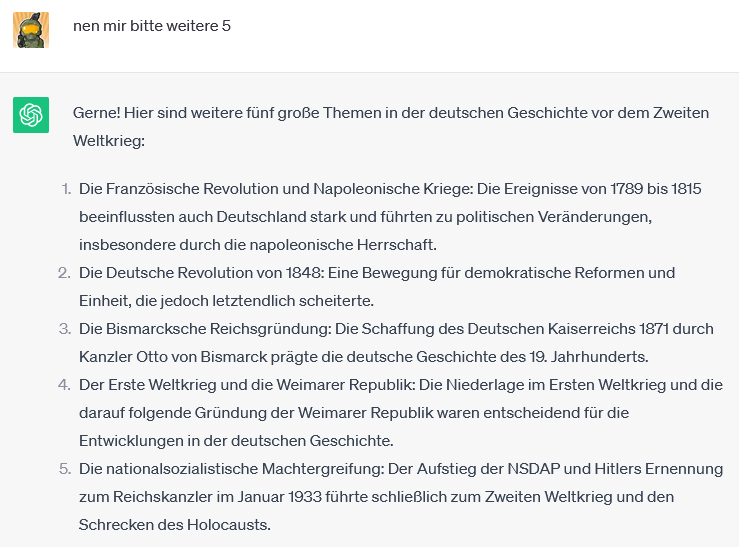
\includegraphics[scale=0.7]{BilderFuerBA/ChatGPT5Themen2.png}
	\caption{Idee 6 bis 10 von ChatGPT}
	\label{fig:Zweiten-Fünf-Idenn}
\end{figure}
\\
Man kann an diesem Beispiel sehen, das ich das Thema in Deutschland, Vor dem zweiten Weltkrieg. und ChatGPT innerhalb dieser Grenze mir 10 eingegrenzt habe.
ChatGPT hat mir in diesem Fall sehr schnell gehlfen mir 10 Ideen zu entwickeln, die ich Thematisch in meinem Videospiel verarbeiten kann. Als Ein-Mann-Videospielentwickler konnte ich mich dann dafür Entscheiden, die Reformation mit Martin Luther als Hauptfigur, zu entscheiden.
Innerhalb dieser Bachlorthesis ist es mir aus zeitgründen nicht möglich ein komplettes Videospiel zu entwickeln was das Leben von Martin Luther wiederspiegelt. Durch meine Recherche über Martin Luther und seinem Leben, fand ich eine Moment sehr bedeutet, und zwar den Moment wo Martin Luther, seine 96 Thesesn an das Kirchtor genagelt hat.
In meinem Prototyp habe ich dieses Ereignes als Thematischen Mittelpunkt gewählt.
Meine Spieleidee für mein Prototyp ist es, das Martin Luther durch ein Dorf Läuft und verschiedene NPCs trifft und mit Ihnen in ein Dialog tritt. Martin Luther trifft verschiedene Personen mit verschiedenen Problemen und Ansichten. Er redet mit Ihnen und lässt sich von ihnen inspirieren. Durch dieser Inspiration entwickelt Martin Luther später im spiel seine 96 Thesen.
Kern meines Prototyp ist eine Spielwert das aus einem Dorf mit mehreren NPCs besteht die einen Dialog mit der Hauptfigur Martin Luther führen kann.


\subsection{Nutzung von KIs zur Erstellung von 2D Bildern}
Als erstes brauche ich eine Spielfigur die Martin Luther nachempfunden ist. Mein Worklfow besteht darin ein Promt von ChatGPT ausgeben zu lassen, den ich Später für Midjourney benutzen kann. Genau diesen Prompt habe ich ChatGPT übergeben.
\\
\begin{figure}[h]
	\centering
	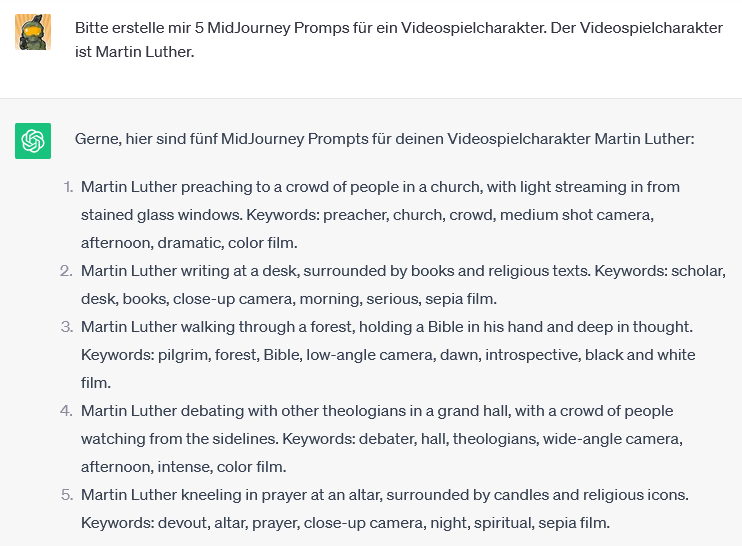
\includegraphics[scale=0.7]{BilderFuerBA/ChatGPTMJML01.png}
	\caption{Idee 3 bis 10 von ChatGPT}
	\label{fig:Prompt-MJ-Fünf-Idenn}
\end{figure}
\\
Man bemerkt, das ChatGPT sehr bemüht ist verschiedene Stimmungen und Situationnen zu beschreiben
\subsection{Nutzung von KIs zur Erstellung von 3D Modellen}
\subsection{Erstellung von Musik und Klängen}
\subsection{Erstellung von Animationen}
\subsection{Entwicklung der Spiellogik}

%5
\section{Ergebnisse und Diskussion}
\subsection{Vorstellung des fertigen Videospiels}
\subsection{Diskussion der Ergebnisse und Einschätzung des Erfolgs des KI-Einsatzes}
\subsubsection{Einsatz von MonsterMash}
	MonsterMash ist ein KI-System mit dem man sehr gut Monster erstellen kann, was der Name auch gut Suggeriert. Wenn man realitätsnahe ergenisse sich Wünscht, wird man mit MonsterMash auf sehr große Herausforderungen treffen. Monster sind Fantasiewesen, und niemand kann genau beschreiben, wie ein Monster aussieht. Bei darstellung von Menschen oder gebäude sieht das anders aus. Für mein Adventure game, mit einem Historischen Hintergrund, ist MonsterMash nicht zu empfehlen. Anders würde es in einem Fantasy-Scenario aussehen, wo undefinierte Gestalten dem Spieler begegnen sollen.
\subsubsection{Einsatz von PFuHD}
PFuHD ist eine KI-System was daruf Trainiert ist Digitalfotos von Personen in ein 3D-Modell umzuwandeln. PFuHD kann man auf Google-Cllab einrichten und lauffähig mahcne. Für mein Projekt habe ich die Demo-Version verwendet, die kostenlos und für meine Zwecke ausreichend war.
Da PIFuHD darauf trainiert war aus Bilder von Personen 3D-Modelle zu erzeugen, habe ich probiert 3D-Modell von Personen zu erstellen lassen, die von Midjourney erzeugt wurden.

Die Kompatibilität zwiwchen Midjourney und PIFuHD war zu meinem überrschen sehr Einfach. Die Resultate waren noch Artefaktbelastetr, was sich besonder in bereichen der Hände und der Robe die Martin Luther trägt verdeutdlicht.

Durch Midjourney konnte ich Bilder von  Martin Luther erzeugen, die als Conzeptgrafiken dienten. Diese Konzeptgraphiken habe ich PIFuHD als eingabe gegeben, und hat mir daraus
\subsection{Kritische Reflexion des Entwicklungsprozesses und Ausblick auf mögliche zukünftige Entwicklungen}

%6
\section{Fazit}
\subsection{Zusammenfassung der Ergebnisse}
\subsection{Implikationen für die Praxis}
\subsection{Limitationen der Studie}

%7
\section{Literaturverzeichnis}

%8
\section{Anhang}
\subsection{Abbildungen und Diagramme}
\subsection{Code-Beispiele}
\subsection{Weitere Materialien}
\end{document}